\documentclass{article}

\usepackage{SIunits}
\usepackage{graphicx}
\usepackage{tikz}
\usepackage{pgfplots}

\usepgfplotslibrary{dateplot}
\usepgfplotslibrary{units}
\usetikzlibrary{external}
\tikzexternalize
\pgfplotsset{compat=1.14}

\begin{document}
\tikzsetnextfilename{fig_rosetta2005_newnorcia}
\tikzset{external/force remake}
\begin{tikzpicture}

\node (morley) at (0,0) {
	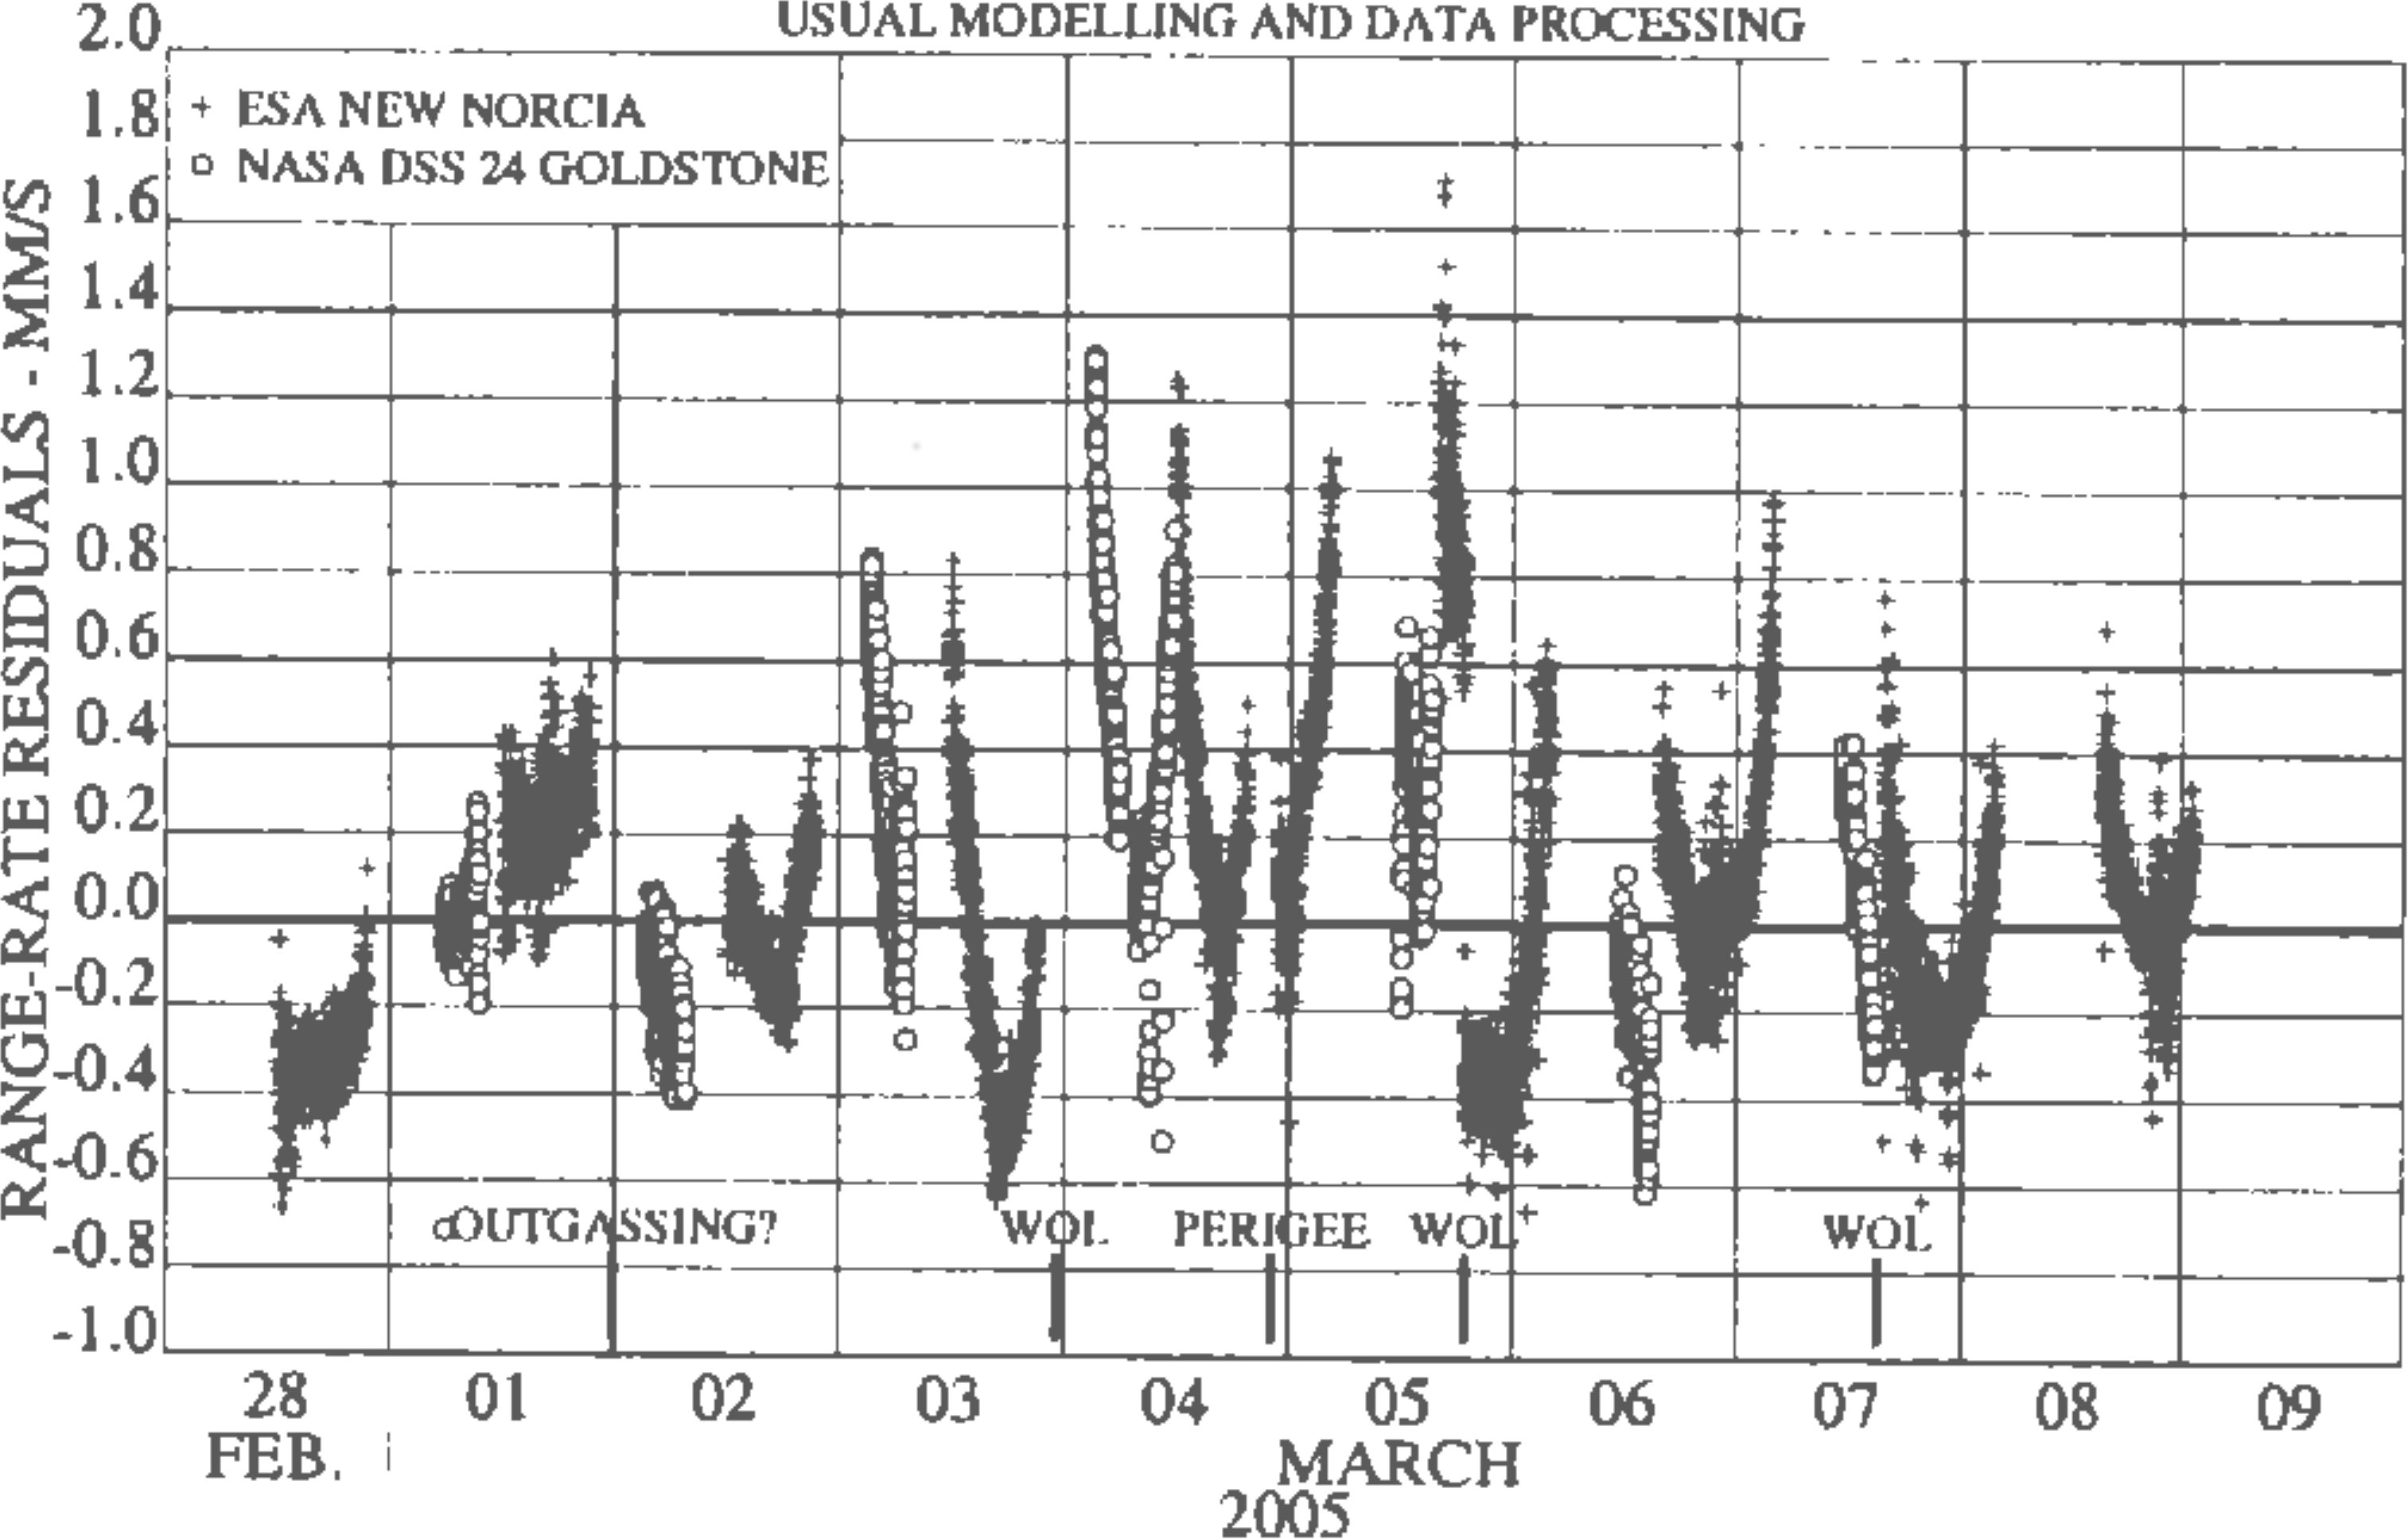
\includegraphics[angle=0.277,width=0.9\textwidth]{Figs/rosetta2005-residuals.png}
	};

\node (jplh) at (0.35, 0.055) {%
	\begin{tikzpicture}[xscale=1.475,yscale=1.035]
	\footnotesize
	\begin{axis}[
		scaled ticks=false,
		axis line style = {red},
		date coordinates in=x,
		date ZERO = 2005-02-28,
		tick align = inside,
		xmin = {2005-02-28 00:00:00},
		xmax = {2005-03-09 23:59:59},
		xticklabel = \empty,
		xtick pos = left,
		ytick style = {draw = none},
		yticklabel = \empty,
		ylabel = {},
		legend style={
			at = {(0.60,0.95)},
			anchor = west,
			draw = none,
			font = \tiny,
			fill = white
			}
		]
		\addplot [thick, mark = none, red]
			table [x index=0, y index=5, col sep=tab, skip first n=1]
			{rosetta2005_newnorcia.t}
		;
		\addlegendentry[red] {Range rate $v$};
	\end{axis}
	\begin{axis}[
		scaled ticks=false,
		axis line style = {blue},
		date coordinates in=x,
		date ZERO = 2005-02-28,
		tick align = inside,
		xmin = {2005-02-28 00:00:00},
		xmax = {2005-03-09 23:59:59},
		xtick pos = left,
		xticklabel = {\tiny \month/\day},
		xticklabel style = {anchor = south, blue},
		ytick style = {draw = none},
		yticklabel = \empty,
		ylabel = {},
		y filter/.code = {\pgfmathparse{0.5-45*(\pgfmathresult)}},
		restrict y to domain = -1.0:3.0,
		legend style={
			at = {(0.60,0.90)},
			anchor = west,
			draw = none,
			font = \tiny,
			fill = white
			}
		]
		\addplot [thick, mark = none, blue]
			table [x index=0, y index=7, col sep=tab, skip first n=1]
			{rosetta2005_newnorcia.t}
		;
		\addlegendentry[blue] {Acceleration $a$};
	\end{axis}
	\end{tikzpicture}
};
\end{tikzpicture}
\end{document}
